\documentclass[11pt, a4paper]{article}

\usepackage{graphicx}
\usepackage[a4paper,top=3cm,bottom=2cm,left=2cm,right=2cm,marginparwidth=1.75cm]{geometry}
\usepackage[english]{babel}
\usepackage[utf8x]{inputenc}
\usepackage{subfig}
\usepackage{float}
\usepackage{amsmath}
\usepackage{amssymb}
\usepackage{mhchem}
\usepackage{hyperref}
\usepackage{tikz}
\usepackage{cancel}
\usepackage{bm}

\graphicspath{ {./images} }
\newcommand*{\qed}{\hfill\ensuremath{\quad\square}}%
\newcommand*{\rad}{\ensuremath{\,\text{rad}}}
\newcommand*{\R}{\ensuremath{\mathbb{R}}}
\newcommand*{\C}{\ensuremath{\mathbb{C}}}
\renewcommand*{\Re}{\operatorname{Re}}
\renewcommand*{\Im}{\operatorname{Im}}
\renewcommand*{\epsilon}{\varepsilon}
\renewcommand*{\phi}{\varphi}
\renewcommand*{\d}{\text{d}}

\DeclareRobustCommand{\uvec}[1]{{%
  \ifcat\relax\noexpand#1%
    % it should be a Greek letter
    \bm{\hat{#1}}%
  \else
    \ifcsname uvec#1\endcsname
      \csname uvec#1\endcsname
    \else
      \bm{\hat{\mathbf{#1}}}%
     \fi
   \fi
}}

\makeatletter
\renewcommand*\env@matrix[1][*\c@MaxMatrixCols c]{%
  \hskip -\arraycolsep
  \let\@ifnextchar\new@ifnextchar
  \array{#1}}
\makeatother

\newtheorem{theorem}{Theorem}
\numberwithin{equation}{section}
\numberwithin{figure}{section}

%------------------------------------------------
%Templates for images and figures
% \begin{figure}[h]
%   \centering
%   \subfloat[caption 1]{{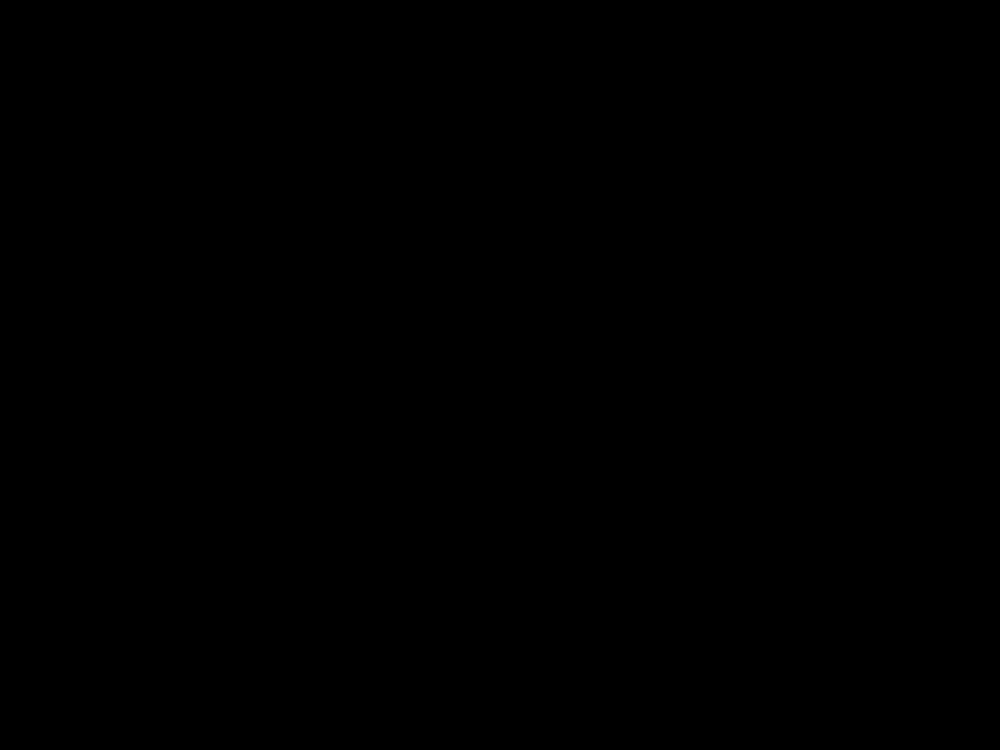
\includegraphics[width=30mm]{images/placeholder.png}}}%
%   \qquad
%   \subfloat[caption 2]{{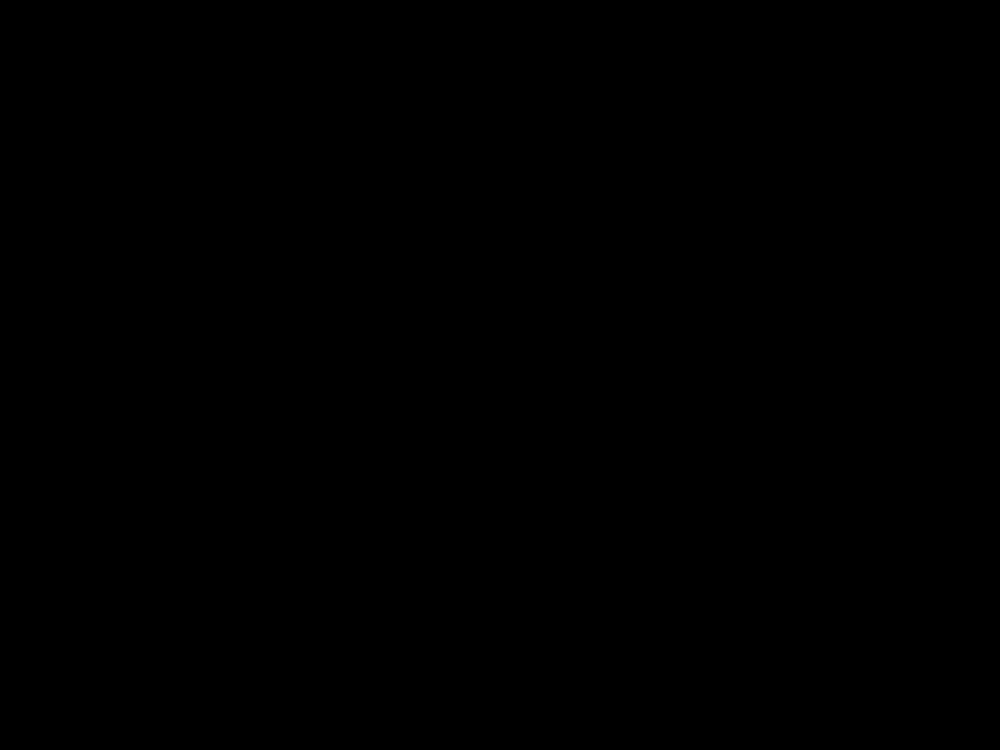
\includegraphics[width=30mm]{images/placeholder.png}}}%
%   \caption{Description}
% \end{figure}

% \begin{figure}[h]
%   \centerline{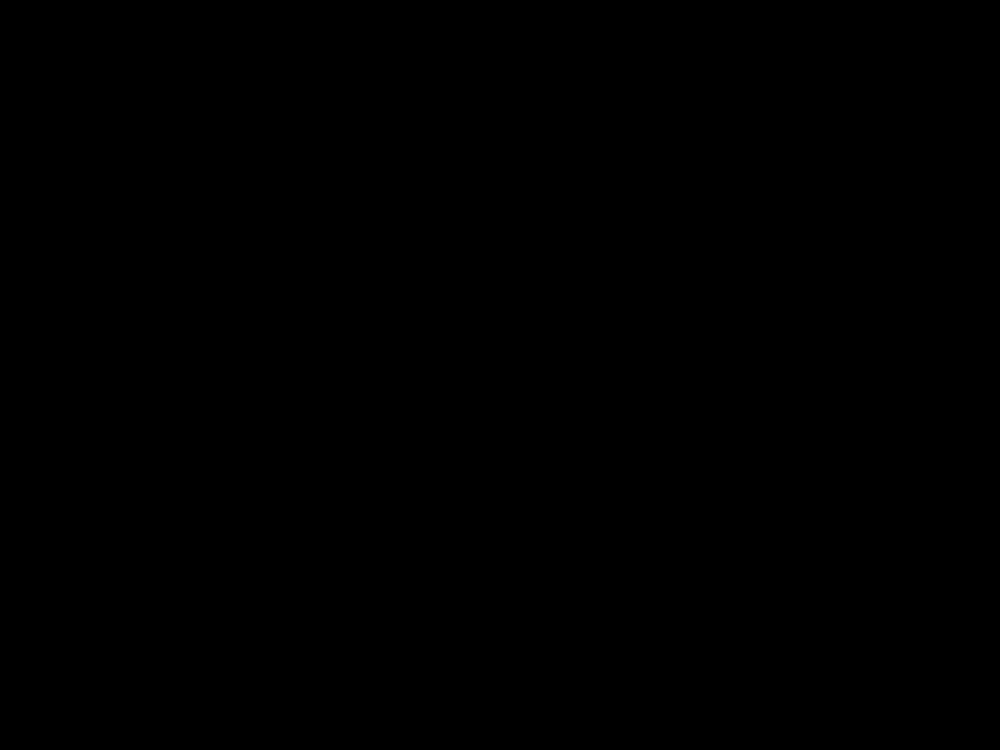
\includegraphics[width=50mm]{images/placeholder.png}}
%   \caption{Description}
% \end{figure}

%Template for a simple table 
%\begin{table}[h]
%   \caption{Description} %title of the table
%   \centering % centering table
%   \begin{tabular}{l rr} % creating three columns
%     \hline\hline %inserting double-line
%     & & \\ [0.5ex] % Insert half line vertical spacing
%     \hline % inserts single-line
%     & & \\ 
%     & & \\
%     & & \\
%     & & \\
%   \hline % inserts single-line
%   \end{tabular}
%   \label{tab:hresult}
% \end{table}
%-----------------------------------------------

\begin{document}
\setcounter{section}{3}

\section{Alternating series}

\subsection{Defining alternating series}
Let $\{ a_n \}$ be a sequence with positive terms. A series constructed from $a_n$ of the form $\sum_{n=1}^\infty (-1)^n a_n$ is called an alternating series because the terms alternate between positive and negative.\\
There are 3 conditions which need to be statisfied for an alternating series to be convergent. Let $\{ b_n \}$ be a sequence which statisfies the following conditions:
\begin{enumerate}
  \item $b_n > 0$ all terms are greater then $0$.
  \item $\lim_{n\to\infty} b_n = 0$, $b_n$ goes to $0$ as $n$ goes to infinity.
  \item $b_n > b_{n+1}$, the sequence is strictly decreasing
\end{enumerate}
If all 3 conditions are met the series $\sum_{n=1}^\infty (-1)^n b_n$ converges.\\
\newline\underline{Example:} Let $b_n$ be a sequence given as:
\begin{equation*}
  b_n = \frac{1}{n+1}
\end{equation*}
Does the series $\sum_{n=1}^\infty (-1)^n b_n$ converge?
\begin{enumerate}
  \item $b_n = \frac{1}{n+1} > 0$ for all $n\geq 0$.
  \item $\lim_{n\to\infty} b_n = \lim_{n\to\infty} \frac{1}{n+1} = 0$
  \item $b_n = \frac{1}{n} > \frac{1}{n+1} = b_{n+1}$
\end{enumerate}
All conditions are statisfies, thus the series converges.

\subsection{Limits of alternating series}
Let $s_n$ be an alternating series for which $s_1 > s_3 > s_5 > \cdots > 0$ and $s_2 < s_4 < s_6 < \cdots < 1$. This means the sequence $s_{2n+1}$ is strictly decrasing and lower bounded by $0$. The sequence $s_{2n}$ is strictly increasing and bounded by $1$. These sequences are both convergent as per the monotomic convergence theorem which states that sequence which are stricly increasing/decreasing and upper/lower bounded always converge. This means:
\begin{gather}
  \lim_{n\to\infty} s_{2n+1} = L\\
  \lim_{n\to\infty} s_{2n} = M
\end{gather}
Since $s_{2n+1}$ and $s_{2n}$ describe the same sequence we know that:
\begin{equation}
  L = M
\end{equation}


\subsection{Estimating remainder terms of alternating series}
The remainder term for an alternating term is found the same as for a regular series. The sum to infinity is the same as the partial sum plus the remainder:
\begin{equation}
  \sum_{n=0}^\infty (-1)^n b_n = \sum_{k=0}^n (-1)^k b_k + R_n
\end{equation}
If $s=\sum_{n=0}^\infty (-1)^n b_n$ is the sum of a sequence which statisfies $b_n > 0$, $b_{n+1} > b_n$ and $\lim_{n\to\infty} b_n = 0$ then the remainder terms is given as:
\begin{equation}
  |R_n| = |s-s_n| \leq b_{n+1}
\end{equation}
\\
\newline\underline{Example:} The following series is given:
\begin{equation*}
  \sum_{n=1}^\infty \frac{(-1)^{n-1}}{n^2} = 1 - \frac{1}{4} + \frac{1}{9} - \frac{1}{16} + \cdots
\end{equation*}
Find for which value of $n$ $R_n < 0.005 = \frac{1}{200}$.
\begin{align*}
  \sum_{k=n+1}^{\infty} \frac{(-1)^{k-1}}{k^2} \Rightarrow |R_n| \leq b_{n+1} &= \frac{1}{(n+1)^2}\\
  \frac{1}{(n+1)^2} &= \frac{1}{200}\\
  n &\approx 14
\end{align*}
Thus the remainder of the series will be smaller then $0.005$ for $n \geq 14$.


\subsection{Absolute and relative convergence}
A series $\sum_{n=1}^\infty a_n$ is absolutely convergent if $\sum_{n=1}^\infty |a_n|$ converges. If the series $\sum_{n=1}^\infty a_n$ converges but the series $\sum_{n=1}^\infty |a_n|$ diverges the series is considered to be a condtionally convergent series.
This means that if the function $\sum_{n=1}^\infty |a_n|$ converges it automatically implies that the series $\sum_{n=1}^\infty a_n$. Any series which is absolutely convergent implies convergence. This does not work the other way around. A convergent series does not automatically implie that the series is absolutely convergent.


\subsection{The ratio test}
Consider the series $\sum_{n=0}^\infty a_n$. Let $\lim_{n\to\infty} \frac{|a_{n+1}|}{|a_n|} = L$. We can conclude the following for different values of $L$:
\begin{itemize}
  \item $L < 1$, $\sum_{n=0}^{\infty} a_n$ is an absolutely convergent series
  \item $L > 1$, $\sum_{n=0}^{\infty} a_n$ is a divergent series
  \item $L = 0$, nothing of significance can be concluded
\end{itemize}
\underline{Example:}
Use the ratio test to determine if the following series converges:
\begin{equation*}
  \sum_{n=1}^{\infty} \frac{(-3)^n}{n!}
\end{equation*}
We apply the theorem:
\begin{align*}
  \lim_{n\to\infty} \frac{|a_{n+1}|}{|a_n|} &= \lim_{n\to\infty} \frac{(-3)^{n+1}}{(n+1)!} \, \Big{/}\, \frac{(-3)^n}{n!}\\
  &=  \lim_{n\to\infty} \frac{(-3)^{n+1}}{(n+1)n!} \, \Big{/}\, \frac{(-3)^n}{n!}\\
  &=  \lim_{n\to\infty} \frac{3}{n+1} = 0 = L < 1
\end{align*}
Thus since $L > 1$ we may conclude that the series is absolutely convergent.


\subsection{The root test}
The root test kinda sucks. $\sum_{n=0}^\infty a_n$ let $\lim_{n\to\infty} \sqrt[n]{|a_n|} = L$, then:
\begin{itemize}
  \item $L < 1$, $\sum_{n=0}^{\infty} a_n$ absolutely converges
  \item $L > 1$, $\sum_{n=0}^{\infty} a_n$ diverges
  \item $L = 0$, nothing of significance can be concluded
\end{itemize}
An important limit that often comes up when dealing with $n$-th roots is:
\begin{equation}
  \lim_{n\to\infty} \sqrt[n]{n} = 1 \Rightarrow \lim_{n\to\infty} \sqrt[n]{n^k} = \lim_{n\to\infty} (\sqrt[n]{n})^k = 1^k = 1
\end{equation}

\end{document}